\label{chapter:preliminary}
En este capítulo haremos un repaso de los conceptos más importantes que nos serán de utilidad a lo largo del trabajo. Recordaremos definiciones y resultados para superficies regulares, enunciaremos y demostraremos el teorema de Brower-Samelson para superficies compactas e introduciremos los entornos tubulares y las superficies paralelas.

\section{Superficies regulares}

\begin{definition}
Un subconjunto $S \subseteq \rtres$, $S \neq \emptyset$, es una \textit{superficie regular} si:

$\forall p \in S$ $\exists V$ entorno abierto de $p$ en $S$ (con la topología inducida de $\rtres$) y una aplicación $X: \utortres$ con $U \subseteq \rdos$ abierto, verificando:

\begin{enumerate}
    \item $X \in \cinf(U, \rtres)$.
    \item $\dxq: \rdostortres$ es inyectiva $\forall q \in \umath$. Dónde $\dxq$ representa la diferencial de $X$ en un punto $q \in U$.
    \item $X(U) = V$ y $X:\utov$ es un homeomorfismo.
\end{enumerate}
\end{definition}

Dada una superficie $S$ y un punto $p \in S$, representaremos por $T_pS$ al plano tangente de $S$ en $p$.

Sea $S \subseteq \rtres$ una superficie. Un \textbf{campo de vectores} (diferenciable) en $S$ es una aplicación diferenciable $\vmath: S \longrightarrow \rtres$. Si $\vmath_p := \vmath(p) \in T_p S$ para todo $p \in S$, diremos que $\vmath$ es un \textbf{campo tangente} a $S$. Si $\vmath_p \bot T_p S$ para todo $p \in S$, diremos que $\vmath$ es un \textbf{campo normal} a $S$. Un \textbf{campo unitario} es aquel que cumple $|\vmath_p| = 1$ para todo $p \in S$.

Se dice que $S$ es una \textbf{superficie orientable} si admite un campo normal unitario global $N: S \longrightarrow \unitsphere$, donde $\unitsphere$ es la esfera unidad en $\rtres$. A este campo $N$ se le llama \textbf{aplicación de Gauss}.

Se llama \textbf{endomorfismo de Weingarten} de $S$ en $p$ al endomorfismo: $A_p = -(dN)_p: T_pS \longrightarrow T_pS$

\begin{definition}[Formas fundamentales]
La \textbf{primera forma fundamental} de $S$ en $p$ es $I_p: T_pS \times T_pS \longrightarrow \rmath$ dada por: 

\begin{equation*}
    I_p(u,v) =  \langle u,v \rangle \qquad \forall u,v \in T_p
\end{equation*}

La \textbf{segunda forma fundamental} de $S$ en $p$ es la forma bilineal $II_p = \sigma_p: T_pS \times T_pS \longrightarrow \rmath$ dada por: 

\begin{equation*}
    \sigma(u,v) = \langle A_p(u),v \rangle  = I_p(A_p(u),v) = - \langle (dN)_p(u), v \rangle \quad \forall u,v \in T_pS
\end{equation*}

\end{definition}

Es sabido que $\sigma_p$ es simétrica y, por tanto, el endomorfismo de Weingarten $A_p$ es autoadjunto.

Como $A_p$ es autoadjunto, entonces es diagonalizable mediante una base ortonormal. En particular, $\exists k_1(p), k_2(p) \in \rmath$, $k_1(p) \leq k_2(p)$, $\exists \{e_1,e_2\}$ base ortonormal en $(T_pS, I_p)$ de forma que $A_p(e_i) = k_i(p)e_i$, $\forall i = 1,2$.

Los números $k_i(p)$ se llaman \textbf{curvaturas principales} de $S$ en $p$.
Los vectores propios no nulos de $A_p$ se llaman \textbf{direcciones principales} de $S$ en $p$.
Se define la \textbf{curvatura de Gauss} de $S$ en $p$ como el número real 
%
\begin{equation*}
    K(p)=det A_p=k_1(p)k_2(p)
\end{equation*}

Se define la \textbf{curvatura media} de $S$ en $p$ como el número real 

\begin{equation*}
    H(p)=\frac{1}{2}tr A_p=\frac{k_1(p)+k_2(p)}{2}
\end{equation*}

Se dice que $S$ es \textbf{una superficie llana} si $K(p)=0$, $\forall p \in S$

\begin{definition}[Superficie totalmente umbilical]
Un punto $p$ es \textbf{umbilical} si $k_1(p)=k_2(p)$.
Se dice que una superficie $S$ es \textbf{totalmente umbilical} si todos son puntos son umbilicales. Esto es equivalente a $H(p)^2=K(p)$.
\end{definition}

\begin{theorem}[Clasificación de las superficies totalmente umbilicales]\label{umbilicaltheorem}
Sea $S \subseteq \rtres$ superficie conexa, cerrada y totalmente umbilical. Entonces es un plano o una esfera.
\end{theorem}

La prueba de este resultado se realizó en la asignatura de curvas y cuperficies.

\begin{lemma}
Sea $S$ una superficie compacta y $F: S \longrightarrow \rtres$ una aplicación diferenciable e inyectiva tal que $(dF)_p: T_pS \longrightarrow \rtres$ es inyectiva $\forall p \in S$. Entonces, $S' = F(S)$ es una superficie y $F: S \longrightarrow S'$ es un difeomorfismo. 
\end{lemma}
\begin{proof}
Sabemos que $F$ es continua, $S$ compacta y $\rtres$ es un espacio de Hausdorff, entonces $F: S \longrightarrow \rtres$ es cerrada, luego $F: S \longrightarrow S'$ es continua, cerrada y biyectiva, es decir, un homeomorfismo.

Veamos que $S'$ es una superficie. Sea $q \in S'$ y $p \in S$ tal que $F(p)=q$. Como $S$ es una superficie, existe una parametrización $X: U \longrightarrow S$ tal que $V = X(U)$ es un entorno abierto de $p$ en $S$. Tomando $V'=F(V)$ tenemos un entorno abierto de $q$ en $S'$. Definimos $X': U \longrightarrow \rtres$ como $X'=F \circ X$. Usando que $(dF)_p$ es inyectiva tenemos que $X'$ define una parametrización de $S'$. Además, es claro que $X'(U) = V'$.
Finalmente, veamos que $F: S \longrightarrow S'$ es un difeomorfismo. Como es biyectiva y diferenciable, bastará ver que su diferecial es un isomorfismo para todo $p \in S$. Sea $p\in S$ y $(dF)_p: T_pS \longrightarrow T_{F(p)}S'$, es claro que $(dF)_p$ es un isomorfismo por tratarse de un monomorfismo entre dos planos vectoriales. Esto conluye la prueba.
\end{proof}

\section{Diferenciación en $S \times I$}

Veamos algunos resultados básicos para las funciones diferenciables que salen de $S \times I$ con $I$ un intervalo.

\begin{definition}[Función diferenciable]
Sea $S$ una superficie y $I \subset \rmath$ un intervalo abierto. Diremos que una función $F: S \times I \longrightarrow \rmath^n$ es \textbf{diferenciable} si para cualquier parametrización $X: U \longrightarrow S$ de $S$, la composición $F \circ (X\times id_I): U \times I \longrightarrow \rmath^n$ es diferenciable en el sentido de Lebesgue.
\end{definition}

\begin{definition}[Diferencial]
Sea $F: S \times I \longrightarrow \rmath^n$ una función diferencial. Para cada $(p,t) \in S \times I$ se define la \textbf{diferencial de $F$} en $(p,t)$ como la función $(dF)_{(p,t)}: T_pS \times \rmath \longrightarrow \rmath^n$ dada por:
%
\begin{equation*}
    (dF)_{(p,t)}(v,a) = \diff{}{s}{s=0} F \big( \alpha(s), t+sa \big), \quad \forall v \in T_pS, \, a \in \rmath
\end{equation*}
\end{definition}

\begin{proposition}
Sea $F: S \times I \longrightarrow \rmath^n$ diferenciable, se define para cada $t\in I$, $F_t: S \longrightarrow \rmath^n$ dada por $F_t(p) = F(p,t)$ para todo $p \in S$. Entonces, $F_t$ es diferenciable para todo $p \in S$.
\end{proposition}

\begin{theorem}[Teorema de la función inversa]
Sea $F: S \times I \longrightarrow \rtres$ una función diferenciable y $(p_0,t_0) \in S \times I$ tal que $(dF)_{(p_0,t_0)} : T_{p_0}S \times \rmath \longrightarrow \rtres$ es un isomorfismo linear. Entonces existe $V$ un entorno abierto de $p_0$ en $S$, $\epsilon > 0$ y un entorno abierto de $F(p_0, t_0)$ en $\rtres$ tal que $F \big( V \times (t_0-\epsilon, t_0+\epsilon) \big) \subset W$ y:
%
\begin{equation*}
    F_{|V \times (t_0-\epsilon, t_0+\epsilon)}: V \times (t_0-\epsilon, t_0+\epsilon) \longrightarrow W
\end{equation*}
%
es un difeomorfismo.
\end{theorem}

Las demostraciones de este teorema y la proposición previa son sencillas.

\section{Teorema de Brower-Samelson}

En esta sección vamos a dar los preliminares necesarios para la demostración del teorema de Brower-Samelson. Comenzaremos con el teorema de Jordan-Brower, que nos permitirá hablar del volumen encerrado por una superficie compacta y terminaremos el capítulo con la definición y propiedades de los entornos tubulares.

Cómo ya sabemos por el teorema de Jordan clásico en el caso de $\rdos$, una curva cerrada y simple, divide el plano en dos regiones conexas, una de ellas acotada.

\begin{theorem}[Teorema de separación de Jordan-Brower]
Sea $S \subseteq \rtres$ una superficie compacta y conexa. Entonces $\rtres - S$ tiene exactamente dos componentes conexas cuya frontera común es $S$.
\end{theorem}

Una demostración de este teorema puede verse en el capítulo 4 de \cite{montielrosbook}.

El teorema de Jordan-Brower es una extensión de este resultado para el caso de $\rtres$. De hecho, esta generalización, cuya prueba se escapa del objetivo de este trabajo, es válida para toda hipersuperficie compacta en $\mathbb{R}^n$, véase en \cite{paperchicago}.

A partir de este teorema, es sencillo probar que una de las componentes está acotada y la otra no. Sea $B$ una bola conteniendo a la superficie $S$, entonces su complemento $\rtres - B$ es un conexo contenido en $\rtres - S$. Por tanto, está dentro de una de sus componente conexas, $C_1$ o $C_2$. Suponiendo que $\rtres - B \subset C_2$, entonces $C_2$ es la componente no acotada y $C_1 \cup S \subset \rtres - C_2 \subset B$ que es acotada. 

\begin{definition}[Dominios interior y exterior]
Llamamos \textbf{dominio interior} y lo denotamos como $\Omega$ a la componente conexa acotada limitada por la superficie compacta $S$. Llamamos \textbf{dominio exterior} a la componente no acotada $\rtres - \Omega=\Omega_{*}$.
\end{definition}

\begin{lemma}
Sea S una superficie y $p \in S$. Existe $W \subset \rtres$ entorno abierto y conexo de $p$ y $\exists G: W \longrightarrow B$ difeomorfismo que cumple $G(W\cap S) = B\cap P$ con $B$ una bola abierta y $P$ un plano, ambos de $\rtres$.
\end{lemma}

La demostración de este lema puede verse en el lemma 4.1 de \cite{montielrosbook}.

\begin{definition}
Sea $S$ superficie conexa y compacta, $p \in S$ y sea $v \in (T_pS)^{\perp}$ con $|v|=1$. Consideremos la recta afín $\alpha: \mathbb{R} \longrightarrow \rtres$ definida como $\alpha(t) = p + tv$. Entonces, $\alpha$ es regular con $\alpha(0)=p$ y $\alpha'(0) = v$. Existe entonces un $\epsilon  >  0$ tal que $\alpha(-\epsilon, \epsilon) \cap S = \{p\}$, veáse remark 4.3 de \cite{montielrosbook} para una demostración. Así, los conexos $\alpha(-\epsilon, 0)$ y $\alpha(0, \epsilon)$ están contenidos en $\rtres - S$. Diremos que $v$ es \textbf{interior} si $\alpha(0, \epsilon) \subset \Omega$; en caso contrario diremos que es \textbf{exterior}. Cuando $v$ es interior se cumple también que $\alpha(-\epsilon, 0) \subset \Omega_*$.
\end{definition}

Con estos preliminares, estamos en condiciones de demostrar el teorema de Brower-Samelson.

\begin{theorem}[Teorema de Brower-Samelson]\label{browersamelson}
Toda superficie compacta $S \in \rtres$ es orientable.
\end{theorem}
\begin{proof}
La idea de esta demostración es construir una orientación de $S$. Para ello comencemos viendo que dado $p \in S$ y $v \in (T_pS)^{\bot}$ con $|v|=1$ tenemos que $v$ es interior o bien $-v$ es interior. Además, no pueden darse a la vez ambas cosas.

Supongamos que $v$ no es interior, luego por definición, $\alpha(\epsilon, 0) \subset \Omega^{*}$ con $\alpha$ la recta afín considerada en la definición previa. Consideremos ahora la recta afín $\beta: \mathbb{R} \longrightarrow \rtres$ dada por $\beta(t)=p + t(-v)$. Luego $\beta(0, \epsilon) = \alpha(-\epsilon, 0) \subset \Omega$ y por tanto $-v$ es interior. Ya hemos probado que si $v$ no es interior, lo es $-v$, veamos ahora que no pueden serlo ambos. 

Supongamos que $v$ y $-v$ son interiores. Esto implicaría que $\alpha(0,\epsilon) \subset \Omega$ y $\beta(0, \epsilon) = \alpha(-\epsilon, 0) \subset \Omega$, lo que contradice que $\alpha(-\epsilon, 0) \subset \Omega_*$.

Tomemos ahora $v \in (T_pS)^{\bot}$ con $|v|=1$ interior (si no fuese interior, tomamos $-v$). Vamos a buscar un entorno abierto $V$ de $p \in S$ para construir una orientación $N: V \longrightarrow \rtres$ con $N(q)$ interior $\forall q \in V.$

Por el lema previo, tenemos que $\exists W$ entorno abierto y conexo de $p$ en $\rtres$ y $G: W \longrightarrow B$ difeomorfismo. Definimos el entorno $V=W\cap S$ entorno de $p$ que es conexo por ser homeomorfo a $B\cap P$. Además, como toda superficie es orientable localmente, podemos suponer que $V$ es orientable.

Sea $N: V \longrightarrow \rtres$ la orientación de $V$ tal que $N(p)$ es interior. Vamos a denotar como $\tilde{\Omega}$ a la componente conexa de $B-P$ tal que $G(W\cap P) = \tilde{\Omega}$ y sea $n \in \rtres$ el normal unitario que apunta hacia $\tilde{\Omega}$.

Definimos la función $f: V \longrightarrow \rmath$ como 
%
\begin{equation*}
    f(q) = \langle (dG)_q(N(q)), n \rangle = \langle \beta'_q(0), n \rangle
\end{equation*}
%
donde $\beta_q(t) = G(q + tN(q))$.

Como $N(q) \not\in T_qS$ y los difeomorfismos conservan la transversalidad se tiene que $\beta'_q(0) \not\in T_{G(p)}P = n^\perp$. En particular, $f(q)$ nunca se anula en $V$. Por continuidad y conexión tenemos tenemos que se conserva el signo:

\begin{align*}
    signo(f(q)) = signo(f(p)) &= signo(\langle (dG)_q(N(q)), n \rangle) \\  &= signo(\langle \beta'_q(0), n \rangle)
\end{align*}

Veamos que este signo es positivo. Tenemos que $\alpha_p(0, \epsilon_p) \subset \Omega$ donde $\alpha_q(t) = q + tN(q)$. Así, $\beta_p(0, \epsilon_p) \subset \tilde{\Omega}$ y, por tanto, $\langle \beta_p(t), n \rangle > 0$, para todo $t \in (0, \epsilon_p)$. Como $\langle \beta_p(0), n \rangle = 0$, derivando, se tiene:

\begin{equation*}
    \diff{}{t}{t=0} \langle \beta_p(t), n \rangle \geq 0 \Rightarrow \langle \beta'_p(0), n \rangle \geq 0
\end{equation*}
%
Por otro lado, como $f$ nunca se anula:
%
\begin{equation*}
    \langle \beta'_p(0), n \rangle > 0
\end{equation*}

Ya hemos probado que el signo es positivo. Veamos que $f(q) > 0$, $\forall q \in V$ lo que implica que $N(q)$ es interior, $\forall q \in V$. Hagámoslo por reducción al absurdo. 

Supongamos que no ocurre, entonces $\exists q \in V$ tal que $N(q)$ no es interior. Entonces se tiene que $\alpha_q(0, \epsilon_q) \subset \Omega_*$ y, por tanto, $\beta_q(0, \epsilon_q) \subset \tilde{\Omega}_*$. Tendríamos que $\langle \beta_q(t), n \rangle < 0$, para todo $t \in (0, \epsilon_q)$ y $\langle \beta_q(0), n \rangle = 0$. Por tanto, análogo al razonamiento anterior, podríamos obtener que $f(q) = \langle \beta'_q(0), n \rangle < 0$ y esto es una contradicción.

Finalmente, definimos $N: S \longrightarrow \rtres$ tal que para cada $p\in S$, $N(p)$ es el único vector normal unitario a $S$ en $p$ que además es interior. Con lo visto anteriormente, sabemos que $N$ es diferenciable y por tanto $S$ es orientable.
\end{proof}

\begin{remark}
Para una superficie compacta y conexa $S$, tomaremos siempre por defecto la aplicación de Gauss interior.
\end{remark}

\section{Entornos tubulares}

En esta sección, vamos a definir los entornos tubulares. Veremos que dada una superficie, bajo determinadas hipótesis, existe un entorno que envuelve la superficie.

Sea $S$ una superficie de $\rtres$. Como $\rtres$ es un espacio métrico, los entornos más sencillos de considerar son los \textbf{entornos métricos}, definidos como los puntos cuya distancia a la superficie es menor que un delta dado. Dado $\delta>0$ denotamos:
%
\begin{equation*}
    B_\delta(S)=\{p\in \rtres \quad | \quad dist(p,S) < \delta\}
\end{equation*}
%
donde, $dist(p,S) = \displaystyle\inf_{q\in S}|p-q|$.

\begin{lemma}
Dada una superficie cerrada $S$ de $\rtres$, el conjunto $B_\delta(S)$ definido anteriormente coincide con el conjunto $N_\delta(S)=\displaystyle\cup_{p\in S}N_\delta(p)$, definido como la unión de los segmentos abiertos en las rectas afines normales a la superficie S con centro $p \in S$ y radio $\delta > 0$.
\end{lemma}
\begin{proof}
Veámoslo por doble inclusión:

Sea $p \in S$, y sea $q \in N_\delta(p)$. Es directo que, $dist(q,S) \leq |q-p| < \delta$, luego $q \in B_\delta(S)$.

Supongamos ahora $q \in B_\delta(S)$. Tomamos la función distancia al cuadrado del punto $q$ a $S$. Como $S$ es cerrado, sabemos que existe un mínimo en un punto $p \in S$. Además por la caracterización de los puntos críticos de la función distancia al cuadrado, sabemos que el punto $q$ está en la recta normal a $S$ en el punto $p$. Así, $|p-q| = dist(q,S) < \delta$, luego $q \in N_\delta(p)$.
\end{proof}

Sea $S$ una superficie orientable con aplicación de Gauss $N: S \longrightarrow \mathbb{S}^2$. Definimos:

\begin{align*}
    F: S \times \mathbb{R} &\longrightarrow \rtres \\
    (p,t) &\longrightarrow p + tN(p)
\end{align*}

Esta aplicación, claramente diferenciable, envía cada par $(p,t)$ a un punto sobre la recta afín normal de $S$ en $p$ a distancia $|t|$. Luego tenemos:

\begin{equation*}
    F(S \times (-\delta, \delta)) = N_\delta(S)=\cup_{p\in S} N_\delta(p), \qquad \forall \delta > 0.
\end{equation*}

\begin{definition}[Entornos tubulares]
La unión $N_\delta(S)$ de todos los segmentos normales de radio $\delta > 0$ centrados en los puntos de una superficie $S$ orientable es llamada \textbf{entorno tubular} de radio $\delta$ si es un abierto como subconjunto de $\rtres$ y la función $F: S \times (-\delta, \delta) \longrightarrow N_\delta(S)$ definida previamente es un difeomorfismo.
\end{definition}

\begin{figure}[h]
  \centering
  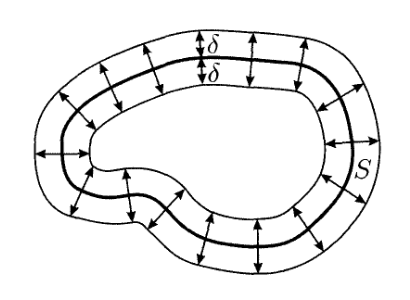
\includegraphics[width=0.9\textwidth]{gfx/tubular_neighbourhoods.png}
  \caption{Entorno tubular}
\end{figure}

\begin{lemma}
Sea $S$ una superficie. Para cada $p \in S$, $\exists V_p$, entorno abierto orientable de $p$ en $S$ y $\delta > 0$ de forma que el conjunto $N_\delta(V_p)$ es un entorno tubular de $V_p$.
\end{lemma}
\begin{proof}
Vamos a empezar la demostración calculando la diferencial de $F$ en un punto $(p,t) \in S \times \rmath$. Dado $v \in T_pS$, tenemos:
%
\begin{align*}
    (dF)_{(p,t)}(v,0) &= \diff{}{s}{s=0} F(\alpha(s), t) \\
    &= \diff{}{s}{s=0} \big( \alpha(s) + tN(\alpha(s) \big) \\ 
    &= \alpha'(0) + t(dN)_{\alpha(0)}(\alpha'(0)) \\ 
    &= v + t(dN)_p(v),
\end{align*}
%
donde $\alpha: (-\epsilon, \epsilon) \longrightarrow S$ es una curva con $\alpha(0) = p$ y $\alpha'(0) = v$. 

Por otro lado, tenemos:
%
\begin{align*}
    (dF)_{(p,t)}(0,1) &= \diff{}{s}{s=0} F(p, t+s) \\ 
    &= \diff{}{s}{s=0} \big( p + (t+s)N(p) \big) \\ &= N(p)
\end{align*}
%
En particular, para $t=0$, tenemos:
%
\begin{align*}
    (dF)_{(p,0)}(v,0) &= v, \qquad \forall v \in T_pS \\
    (dF)_{(p,0)}(0,1) &= N(p).
\end{align*}

Por tanto, $(dF)_{(p,0)}$ es un isomorfismo. Concluimos utilizando el teorema de la función inversa, que nos asegura que existe $V_p$ entorno abierto de $p$ en $S$ y $\delta_p > 0$, tal que, $F: V_p \times (-\delta_p, \delta_p) \longrightarrow F(V_p \times (-\delta_p, \delta_p))$ es un difeomorfismo. Además, como toda superficie $S$ es orientable localmente, se puede suponer que $V_p$ es orientable.
\end{proof}

Veamos ahora la existencia de entornos tubulares para superficies compactas, utilizando el lema previo para demostrarlo.

\begin{theorem}[Existencia de entornos tubulares]
Sea $S$ una superficie orientable y $R \subset S$ un subconjunto abierto relativamente compacto. Entonces $\exists \epsilon > 0$ tal que el conjunto $N_\epsilon(R)$ es un entorno tubular de la superficie $R$, esto es, es un abierto de $\rtres$ y la función:

\begin{align*}
    F: R \times (-\epsilon, \epsilon) &\longrightarrow N_\epsilon(R) \\
    (p,t) &\longrightarrow p + tN(p)
\end{align*}
%
es un difeomorfismo.

En particular, cuando la superficie $S$ es compacta, $\exists \epsilon > 0$ tal que
$B_\epsilon(S)=N_\epsilon(S)$ es un entorno tubular de $S$.
\end{theorem}
\begin{proof}
Como $\overline{R}$ es compacto, existe por el lema previo un recubrimiento finito por abiertos de $\overline{R}$ cada uno con un entorno tubular. Sea $\delta > 0$ el menor radio de todos ellos. La función $F$ definida previamente restringida a $R \times (-\delta, \delta)$ es un difeomorfismo local. Vamos a buscar un $\epsilon \in (0,\delta)$ tal que la función $F$ restringida a $R \times (-\epsilon, \epsilon)$ es inyectiva. Veámoslo por reducción al absurdo.

Supongamos que $\forall \epsilon \in (0,\delta)$ se cumple que $F$ restringida al intervado de definición $R \times (-\epsilon, \epsilon)$ no es inyectiva, o lo que es lo mismo, los segmentos normales $N_\epsilon(p)$ con $p \in R$ intersecan entre ellos. Así, dado $\epsilon=\frac{1}{n}$ con $n \in \mathbb{N}$, $\exists p_n,q_n \in S$ con $p_n \neq q_n$ tal que $N_{\frac{1}{n}}(p_n) \bigcap N_{\frac{1}{n}}(q_n) \neq \emptyset$.
Como $R$ es relativamente compacto, podemos tomar sucesiones parciales que convergen en $\overline{R}$. Sean $\{p_n\}_{n \in \mathbb{N}}, \{q_n\}_{n \in \mathbb{N}}$ estas sucesiones y sean $p,q \in \overline{R}$ los puntos donde convergen, esto es:

\begin{equation*}
    \lim_{n\to\infty} p_n = p \qquad \lim_{n\to\infty} q_n = q
\end{equation*}

Dado $r_n \in N_{\frac{1}{n}}(p_n) \bigcap N_{\frac{1}{n}}(q_n)$, entonces:

\begin{equation*}
    |p_n - q_n| = |p_n - q_n + r_n - r_n| \leq |p_n-r_n| + |r_n-q_n| < \frac{1}{n}+\frac{1}{n} = \frac{2}{n}
\end{equation*}

Por tanto los límites coinciden, es decir, $p=q$.

Aplicando el lema previo al punto $p = q \in S$, tenemos $V$ entorno abierto de $p$ en $S$ y $\rho > 0$ tal que $N_\rho(V)$ es un entorno tubular. Además, $\exists N_0 \in \mathbb{N}$ tal que, $\forall n > N_0$, $p_n,q_n \in V$ y $1/n < \rho$. Por tanto llegamos a una contradicción:
%
\begin{equation*}
    N_{\frac{1}{n}}(p_n) \cap N_{\frac{1}{n}}(q_n) \subset N_\rho(p_n)\cap N_\rho(q_n) = \emptyset
\end{equation*}
%
ya que $N_\rho(V)$ es un entorno tubular y, por tanto, $F$ restringida a $(-\rho, \rho)$ es inyectiva. Hemos probado que $\exists \epsilon \in (0, \delta)$ tal que $F: \rmath \times (-\epsilon, \epsilon) \longrightarrow N_\epsilon(R)$ es un difeomorfismo local inyectivo. Como claramente es sobreyectivo entonces $N_\epsilon(R)$ es un entorno tubular y se termina la prueba.
\end{proof}

A partir de los entornos tubulares, introduciremos el concepto de superficie paralela para concluir el capítulo.

\begin{definition}[Superficie paralela]
Sea $\rho > 0$ y sea $N_\rho(S)$ un entorno tubular de la superficie $S$ compacta con $N$ su aplicación de Gauss. Para todo $t \in (-\rho, \rho)$ se define el conjunto $S_t=\{p + tN(p); p \in S\}$ superficie compacta y la aplicación $F_t: S \longrightarrow S_t$ dada por $F_t(p)=p+tN(p)$ es un difeomorfismo.
Llamamos a $S_t$ \textbf{superficie paralela} a $S$ a una distancia $t$.
\end{definition}